%!TEX TS-program = XeLaTeX
%!TEX TS-program = XeLaTeX
\documentclass[11pt]{article}

\usepackage{amssymb}
\usepackage{amsthm}
\usepackage{amsmath}
\usepackage{mathtools}

\usepackage{fancyhdr}
\usepackage{graphicx}
\usepackage[top=3cm, left=2cm, right=2cm, headheight = 90pt]{geometry}
\usepackage{xltxtra}
\usepackage[font=small,labelfont=bf]{caption}

\usepackage{multicol}

\renewcommand{\theenumi}{\alph{enumi}}


\def\leq{\leqslant}
\def\geq{\geqslant}
\def\N{\mathbb N}
\def\R{\mathbb R}
\def\Z{\mathbb Z}
\DeclarePairedDelimiter\set\{\}

\def\prob{}

\theoremstyle{definition}
\newtheorem{problem}{\prob}


\pagestyle{fancy}

%!TEX TS-program = XeLaTeX

\fancyfoot[CE,CO]{}  % this is to remove page numbers (as you might want for single page docs)

%%!TEX TS-program = XeLaTeX
\renewcommand{\figurename}{Attēls}

\fancyhead[C]{{\Large\bf IMO SL  list 2 geometric combinatorics - Problems}}



\renewcommand{\theenumi}{\alph{enumi}}

\begin{document}

\noindent
 
\filbreak


\begin{problem}
%2014C1 -nice and easy, points within rectangle

Let $n$ points be given inside a rectangle $R$ such that no two of them lie on a line parallel to one of the sides of $R$. The rectangle $R$ is to be dissected into smaller rectangles with sides parallel to the sides of $R$ in such a way that none of these rectangles contains any of the given points in its interior. Prove that we have to dissect $R$ into at least $n - 1$ smaller rectangles.


\end{problem}

\begin{problem}
%2010C3 - ok, chess king positioning

$2500$ chess kings have to be placed on a $100\times 100$ chessboard so that
\begin{itemize}
\item no king can capture any other one (i.e. no two kings are placed in two squares sharing a common vertex);
\item each row and each column contains exactly $25$ kings.
\end{itemize}
Find the number of such arrangements. (Two arrangements differing by rotation or symmetry are supposed to be different.)


\end{problem}


\begin{problem}
%2014C4 - easyish tetraminos

Construct a tetromino by attaching two $2 \times 1$ dominoes along their longer sides such that the midpoint of the longer side of one domino is a corner of the other domino. This construction yields two kinds of tetrominoes with opposite orientations. Let us call them \textit{S-} and \textit{Z-tetrominoes}, respectively.

\begin{center}

\centering
\begin{minipage}{.5\textwidth}
  \centering
  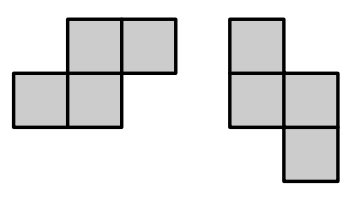
\includegraphics[width=.4\linewidth]{stetramino.png}
  \captionof{figure}{S-tetramino}
  \label{fig:test1}
\end{minipage}%
\begin{minipage}{.5\textwidth}
  \centering
  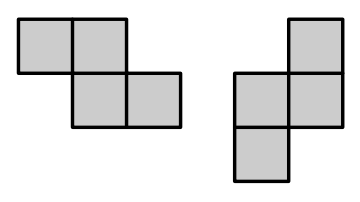
\includegraphics[width=.4\linewidth]{z-tetramino.png}
  \captionof{figure}{Z-tetramino}
  \label{fig:test2}
\end{minipage}

\end{center}



Assume that a lattice polygon $P$ can be tiled with S-tetrominoes. Prove than no matter how we tile $P$ using only S- and Z-tetrominoes, we always use an even number of Z-tetrominoes.

\end{problem}

\begin{problem}
%2014C5 - nice, line coloring
Consider $n \ge 3$ lines in the plane such that no two lines are parallel and no three have a common point. These lines divide the plane into polygonal regions; let $F$ be the set of regions having finite area. Prove that it is possible to colour $\ceil{\sqrt{n/2}}$ of the lines blue in such a way that no region in $F$ has a completely blue boundary. (For a real number $x$, $\ceil{x}$ denotes the least integer which is not smaller than $x$.)

\end{problem}

\begin{problem}
%2011C7 - ok, hardish
On a square table of $2011$ by $2011$ cells we place a finite number of napkins that each cover a square of $52$ by $52$ cells. In each cell we write the number of napkins covering it, and we record the maximal number $k$ of cells that all contain the same nonzero number. Considering all possible napkin configurations, what is the largest value of $k$?

\end{problem}

%
\end{document}
